\documentclass[12pt]{article}
\usepackage[a4paper,margin=1in]{geometry}
\usepackage{enumitem}
\usepackage{graphicx}
\usepackage{hyperref}
\usepackage{longtable}
\usepackage{float}  % To control placement of tables and figures
\title{Lab 3: Building a Mobile App with React Native}
\author{Charitha Vennapusala}
\date{November 17th 2024}
\begin{document}
\maketitle
\section*{Task 1: Set Up the Dev Environment}
\subsection*{(1) Screenshots of Your App}
\begin{figure}[H] 
    \centering
    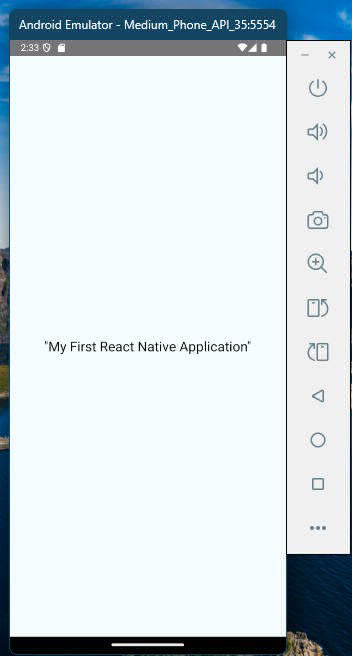
\includegraphics[width=0.6\textwidth, height=9cm]{images/emulator_screenshot.png.png}
    \caption{App running in emulator}
    \label{fig:emulator} 
\end{figure}
\begin{figure}[H] 
    \centering
    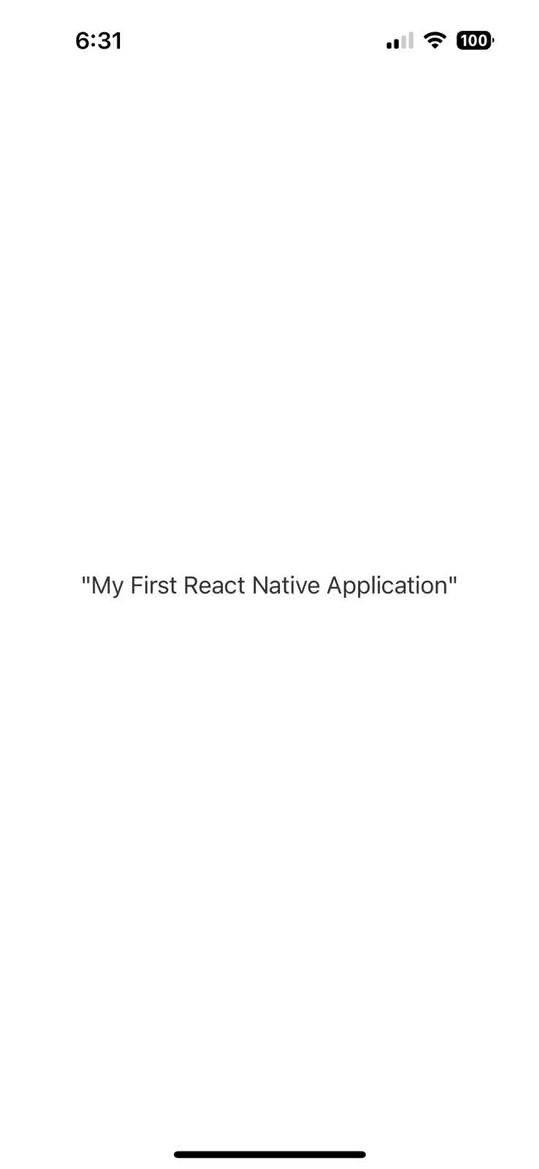
\includegraphics[width=0.7\textwidth, height=9cm]{images/physical_device_screenshot.png.png}
    \caption{App running on a physical device}
    \label{fig:physical_device} 
\end{figure}
\subsection*{Differences Observed}
\textbf{On Emulator:}
\begin{itemize}
    \item Running the app on the Android emulator was quite smooth.
    \item The emulator simulates the device environment and provides a close approximation of how the app would look on a real device.
    \item However, it tends to be slower, especially during startup, and performance might not be as smooth compared to a physical device.
    \item The app displayed correctly but took longer to start due to the emulator’s initialization time.
    \item UI elements looked consistent with how they were coded but might not reflect actual device performance.
    \item Testing was limited to simulated gestures and touch interactions, which may not accurately represent real-world user behavior.
    \item Certain hardware-specific features like GPS and accelerometer are simulated but may not provide reliable results.
    \item The emulator allowed for easy switching between different screen sizes and resolutions, which is useful for testing layouts on various devices.
\end{itemize}
\textbf{On Physical Device:}
\begin{itemize}
    \item Running the app on the physical device was significantly faster.
    \item The app was more responsive, and it felt more like an actual native app.
    \item Expo Go provides a faster, more real-world representation of how the app behaves.
    \item The performance was better, and there were no delays or lag, unlike the emulator.
    \item The real device allowed me to test actual touch interactions and gestures, which felt more natural compared to the emulator.
    \item Real-world testing on a physical device made it possible to evaluate battery usage and power efficiency, which cannot be simulated in an emulator.
    \item It was easier to verify features like camera integration, real GPS data, and push notifications on the physical device.
    \item Debugging real-world issues like connectivity (Wi-Fi/mobile data) was more accurate on a physical device compared to the emulator’s simulated environment.
    \item The display on the physical device provided a true representation of screen resolution, brightness, and color accuracy, which are often scaled on the emulator.
\end{itemize}
\subsection*{(2) Setting Up an Emulator}
\paragraph{Steps to Set Up the Emulator:}
\begin{enumerate}
    \item \textbf{Install Android Studio:} 
    Download and install Android Studio from the official website (\url{https://developer.android.com/studio}).
    \item \textbf{Install Android SDK Tools:}
    \begin{itemize}
        \item Open Android Studio and navigate to \texttt{Settings > Appearance \& Behavior > System Settings > Android SDK}.
        \item Select the \textbf{SDK Platforms} tab and install the latest Android version (e.g., Android 15, API Level 35).
        \item Switch to the \textbf{SDK Tools} tab and install the following tools:
        \begin{itemize}
            \item Android SDK Build-Tools
            \item Android Emulator
            \item Android Emulator hypervisor driver
            \item Android SDK Platform-Tools
            \item Intel x86 Emulator Accelerator (HAXM)
        \end{itemize}
        \item Click \textbf{Apply} to download and install these components.
    \end{itemize}
    \item \textbf{Set Up an Android Virtual Device (AVD):}
    \begin{itemize}
        \item Open the AVD Manager, accessible via \texttt{Welcome Screen > Configure > AVD Manager}, or from the main interface under \texttt{Tools > AVD Manager}.
        \item Create a new virtual device:
        \begin{itemize}
            \item Device: Select \textbf{Medium Phone}.
            \item System Image: Choose a system image for API Level 35.
        \end{itemize}
        \item Configure the AVD:
        \begin{itemize}
            \item Adjust settings to allocate sufficient resources.
            \item Enable hardware acceleration for better performance.
        \end{itemize}
    \end{itemize}
    \item \textbf{Start the Emulator:}
    Launch the emulator using the \textbf{Play} button in the AVD Manager. Wait for the emulator to boot up completely.
\end{enumerate}
\subsection*{Challenges Faced and Solutions:}
\begin{itemize}
    \item \textbf{Slow Performance:} 
    \begin{itemize}
        \item The emulator was initially slow, leading to long app load times.
        \item Enabling hardware acceleration through the Intel HAXM installer resolved the issue.
    \end{itemize}
    \item \textbf{System Image Issues:} 
    \begin{itemize}
        \item Encountered problems downloading the correct system images.
        \item Resolved by ensuring the latest version of Android Studio and proper SDK updates were installed.
    \end{itemize}
    \item \textbf{Internet Access Issues:} 
    \begin{itemize}
        \item At one point, the emulator couldn’t connect to the internet.
        \item Restarting the emulator and checking the AVD network settings fixed the problem.
    \end{itemize}
\end{itemize}
\subsection*{(3) Running the App on a Physical Device Using Expo}
\paragraph{Steps to Connect the Physical Device:}
\begin{enumerate}
    \item \textbf{Set Up Expo:}
    \begin{itemize}
        \item Installed the Expo CLI globally using:
        \begin{verbatim}
npm install -g expo-cli
        \end{verbatim}
        \item Created a new Expo project:
        \begin{verbatim}
npx expo init ExpoProject
cd ExpoProject
npx expo start
        \end{verbatim}
        \item This launched the Expo developer tools in the browser.
    \end{itemize}
    \item \textbf{Install Expo Go on the Physical Device:}
    \begin{itemize}
        \item Downloaded and installed the Expo Go app from the Google Play Store on my Android device.
    \end{itemize}
    \item \textbf{Connect Both Devices:}
    \begin{itemize}
        \item Ensured that my development machine and physical Android device were connected to the same Wi-Fi network.
    \end{itemize}
    \item \textbf{Scan the QR Code:}
    \begin{itemize}
        \item Opened the Expo Go app and used it to scan the QR code displayed in the Expo developer tools on the browser.
        \item The app loaded automatically on the physical device.
    \end{itemize}
    \item \textbf{Modify and Test the App:}
    \begin{itemize}
        \item Made changes to the \texttt{App.js} file to display “My First React Native Application”.
        \item Observed that changes were reflected instantly in the Expo Go app without requiring a rebuild.
    \end{itemize}
\end{enumerate}
\paragraph{Troubleshooting Steps for Physical Device Setup:}
\begin{itemize}
    \item \textbf{App Not Loading:}
    \begin{itemize}
        \item Restarted the Expo server with:
        \begin{verbatim}
npx expo start --clear
        \end{verbatim}
        \item Ensured the Expo Go app was up to date and reinstalled it if necessary.
    \end{itemize}
    \item \textbf{Network Issues:}
    \begin{itemize}
        \item Verified that both devices were on the same Wi-Fi network.
        \item Restarted the router to resolve any connectivity issues.
        \item Used LAN or USB debugging when the Wi-Fi network was unreliable.
    \end{itemize}
    \item \textbf{Cache Problems:}
    \begin{itemize}
        \item Cleared the Metro bundler cache:
        \begin{verbatim}
npx expo start --clear
        \end{verbatim}
        \item Deleted the \texttt{node\_modules} folder and reinstalled dependencies using:
        \begin{verbatim}
npm install
        \end{verbatim}
    \end{itemize}
    \item \textbf{Performance Optimization:}
    \begin{itemize}
        \item Disabled unnecessary processes and apps on the physical device to ensure smooth app performance.
    \end{itemize}
\end{itemize}
\subsection*{(4) Comparison of Emulator vs. Physical Device}
\caption{Comparison between Emulator and Physical Device}
\begin{table}[h!]
\centering
\begin{tabular}{|l|p{6cm}|p{6cm}|}
\hline
\textbf{Aspect} & \textbf{Emulator} & \textbf{Physical Device} \\ \hline
Performance & Slower and less responsive. & Faster and more accurate to real-world performance. \\ \hline
Touch Interaction & Simulated touch gestures may not reflect actual user behavior. & Real touch interactions provide more reliable testing of user experience. \\ \hline
Setup & Requires installation of Android Studio and setup of AVD. & Requires only the Expo Go app and a shared Wi-Fi connection. \\ \hline
Accessibility & Useful for testing various screen sizes and API levels without needing multiple devices. & Limited to the physical device you have access to. \\ \hline
Battery/Hardware Testing & No real hardware interactions, such as battery or camera testing. & Allows testing real-world hardware functionality like sensors, camera, and GPS. \\ \hline
Convenience & Available on the development machine, eliminating the need for additional hardware. & Requires a physical device to be available at all times. \\ \hline
\end{tabular}
\caption{Comparison between Emulator and Physical Device}
\label{tab:emulator_vs_physical_device}
\end{table}
\paragraph{Emulator:}
\textbf{Advantages:}
\begin{itemize}
    \item Provides a close simulation of the device environment, useful for testing different device sizes and Android versions.
    \item Easy to reset and configure with various hardware profiles and system images.
    \item Can be faster for certain development tasks as the app is launched in a controlled environment.
\end{itemize}
\textbf{Disadvantages:}
\begin{itemize}
    \item Performance is slower, especially on lower-end computers, and can be resource-intensive.
    \item May not always reflect real-world app performance due to the lack of actual hardware interactions.
\end{itemize}
\paragraph{Physical Device:}
\textbf{Advantages:}
\begin{itemize}
    \item Offers real-world performance and behavior, including real-time interactions with hardware components like GPS, camera, and sensors.
    \item Provides more accurate testing for responsiveness and app fluidity.
\end{itemize}
\textbf{Disadvantages:}
\begin{itemize}
    \item Requires a physical device that is available and connected via USB or over Wi-Fi.
    \item May not be practical to test every potential device or screen size.
\end{itemize}
\section*{(5)Troubleshooting a Common Error}
\subsection*{Error Encountered}
When I first ran the Expo project on my Android emulator, the app didn’t load, and I got the following error message in the terminal:
\begin{quote}
\textbf{Error:} Unable to connect to development server.
\end{quote}
\subsection*{Cause}
This issue was caused by the emulator not being properly connected to the development server due to network issues or a misconfigured Expo environment.
\subsection*{Steps to Resolve}
\begin{enumerate}
    \item \textbf{Check Network Connection:}  
    I ensured that both my development machine and the Android emulator were connected to the same network.
    \item \textbf{Restart Expo Server:}  
    Running \texttt{npx expo start --clear} helped clear the cache and resolve any server-side issues.
    \item \textbf{Reset Metro Bundler Cache:}  
    Restarting the Metro bundler with \texttt{npx react-native start --reset-cache} cleared stale files and reestablished the development environment.
    \item \textbf{Verify Emulator Settings:}  
    \begin{itemize}
        \item I checked the Android Emulator settings to confirm it had internet access.
        \item Restarting the emulator helped establish a stable connection.
    \end{itemize}
\end{enumerate}
\section*{Task 2: Building a Simple To-Do List App}
\subsection*{(a) Mark Tasks as Complete}
\textbf{Implementation:}  
A toggle function (\texttt{toggleTaskCompletion}) was added to mark tasks as completed or not.  
\begin{itemize}[left=1.5em]
    \item When the user taps on the checkmark, the task's completed status is toggled. This triggers a state update and modifies the task's appearance, reflecting the completion status.
    \item Tasks marked as complete will have a strikethrough on the text (\texttt{textDecorationLine: 'line-through'}) and their color changes to gray (\texttt{color: \#808080}) to indicate completion.
\end{itemize}

\textbf{Screenshots for toggling task completion:}  
\begin{figure}[H]
    \centering
    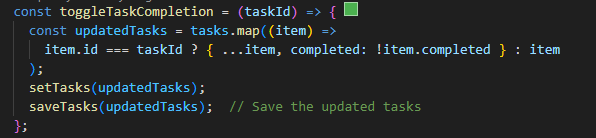
\includegraphics[width=0.8\textwidth]{images/completed1.png} 
    \caption{Screenshot showing the initial list of tasks.}
    \label{fig:toggle-task-1}
\end{figure}
\textbf{Explanation:}
\begin{itemize}[left=1.5em]
    \item The toggleTaskCompletion function maps over the tasks, checking each task's id. When a match is found, it toggles the completed property.
    \item The UI updates automatically because the state is modified and passed into the component's render method, triggering a re-render.
\end{itemize}
\textbf{Visual Outcome:}  
Completed tasks will be displayed with a strikethrough, and their color changes to gray (\#808080) to indicate they are marked as completed.

\begin{figure}[H]
    \centering
    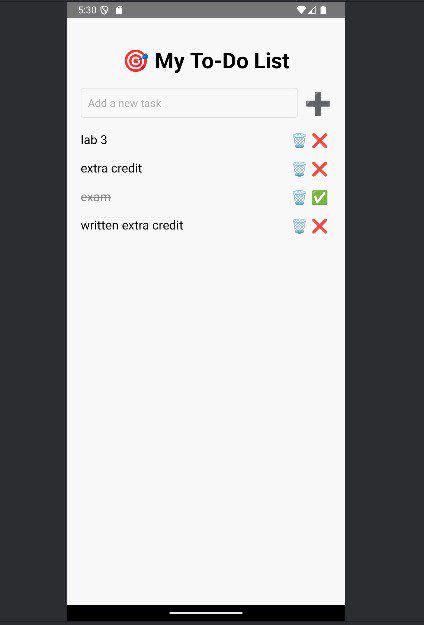
\includegraphics[width=0.4\textwidth]{images/completed3.png} 
    \caption{Screenshot showing a task marked as completed with strikethrough and gray text.}
    \label{fig:toggle-task-2}
\end{figure}


\subsection*{(b) Persist Data Using AsyncStorage }
\textbf{Implementation:}  
\begin{itemize}[left=1.5em]
    \item \texttt{AsyncStorage} was used to persist the list of tasks, ensuring that they are saved across app restarts.
    \item Whenever the tasks array is updated (adding, deleting, or toggling tasks), the updated tasks are saved in \texttt{AsyncStorage}.
    \item On app launch, tasks are retrieved from \texttt{AsyncStorage} and loaded into the state.
\end{itemize}
\textbf{Screenshots for saving and loading tasks:}  
\begin{figure}[H]
    \centering
    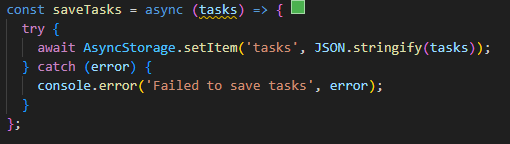
\includegraphics[width=0.8\textwidth]{images/async1.png} 
    \caption{Screenshot showing the tasks being saved.}
    \label{fig:asyncstorage-save}
\end{figure}
\begin{figure}[H]
    \centering
    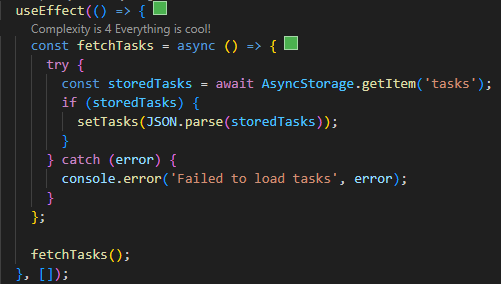
\includegraphics[width=0.8\textwidth]{images/async2.png} 
    \caption{Screenshot showing tasks loaded from AsyncStorage when app start.}
    \label{fig:asyncstorage-load}
\end{figure}
\textbf{Explanation:}  
\begin{itemize}[left=1.5em]
    \item Saving Tasks: Each time the task list changes (add, delete, or update), the tasks are stored in AsyncStorage.
    \item Fetching Tasks: Upon app launch or reload, tasks are fetched from AsyncStorage and set in the state, preserving the user's data.
    \item On app launch, tasks are retrieved from \texttt{AsyncStorage} and loaded into the state.
\end{itemize}
\textbf{Visual Outcome:}  
The tasks will persist across app restarts, maintaining the user's list even if the app is closed and reopened.

\subsection*{(c) Edit Tasks }
\textbf{Implementation:}  
\begin{itemize}[left=1.5em]
    \item Allow users to tap on a task, which will enable an input field for editing the task's text.
    \item After editing, users can submit the changes by pressing Enter.
    \item The state is updated with the modified text, and the updated list of tasks is saved back to \texttt{AsyncStorage}.
\end{itemize}

\textbf{Screenshots for editing tasks:}  
\begin{figure}[H]
    \centering
    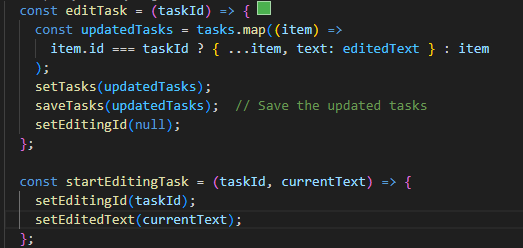
\includegraphics[width=0.7\textwidth]{images/edittask1.png} 
    \caption{Screenshot showing a task in editing mode.}
    \label{fig:edit-task-start}
\end{figure}
\begin{figure}[H]
    \centering
    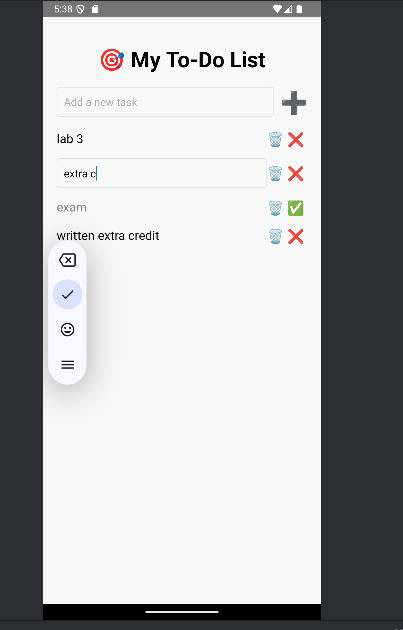
\includegraphics[width=0.5\textwidth]{images/edittask3.png} 
    \caption{Screenshot showing the edited task with updated text.}
    \label{fig:edit-task-complete}
\end{figure}
\textbf{Explanation:}  
\begin{itemize}[left=1.5em]
    \item When the user taps on a task, the startEditingTask function is called, which sets the editingId and shows an input field with the current task text.
    \item After editing the text, the editTask function is triggered to update the task in the state array, and the updated tasks list is saved.
\end{itemize}
\textbf{Visual Outcome:}  
When a task is being edited, the text becomes editable. After editing, the task's text is updated, and the UI reflects the change.

\subsection*{(d) Add Animations}
\textbf{Implementation:}  
\begin{itemize}[left=1.5em]
    \item The \texttt{Animated} API was used to add an animation effect to the “+” button when a new task is added.
    \item The button slightly enlarges when tapped, providing feedback to the user.
    \item The animation effect is triggered using \texttt{Animated.spring} with a friction value to create a bouncing effect when the user taps the add button.
\end{itemize}

\textbf{Screenshots for “Add Task” button animation:}  
\begin{figure}[H]
    \centering
    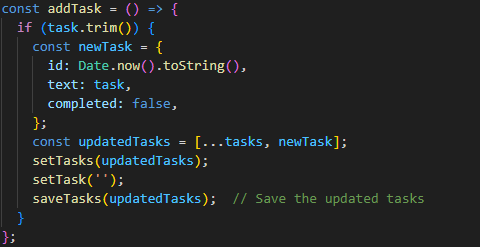
\includegraphics[width=0.8\textwidth]{images/animation2.png} 
    \caption{"Add Task" animation button.}
    \label{fig:add-task-animation-1}
\end{figure}
\begin{figure}[H]
    \centering
    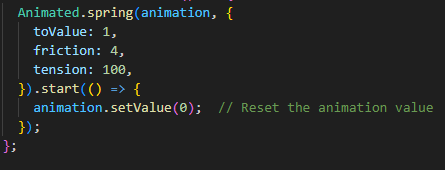
\includegraphics[width=0.8\textwidth]{images/animated3.png} 
    \caption{Trigger the animation.}
    \label{fig:add-task-animation-2}
\end{figure}
\textbf{Explanation:}  
\begin{itemize}[left=1.5em]
    \item The animation value is animated when the user taps the "+" button to add a new task. The spring animation provides a bouncing effect, and once completed, the animation value resets to 0.
\end{itemize}
\textbf{Visual Outcome:}  
The “+” button for adding tasks features an animation effect, providing a more engaging user experience.

\section*{GitHub Repository}
The source code for this project can be found on GitHub: 
\href{https://github.com/VennapusalaCharitha/SimpleTodoApp.git}{\textbf{GitHub Repository Link}}.

\end{document}





